\newpage
\section{Appendix}
%\thispagestyle{empty}
%\pagenumbering{Roman} 	% R XI and r xi
%\addcontentsline{toc}{section}{Appendix}

%%% table settings
\setcounter{table}{0}
\renewcommand{\thetable}{A\arabic{table}}

\setcounter{figure}{0}
\renewcommand{\thefigure}{A\arabic{figure}}

\small

\begin{figure}[!th]
	\caption{Heatmap of all Variables Used}
	\label{heatmap}
	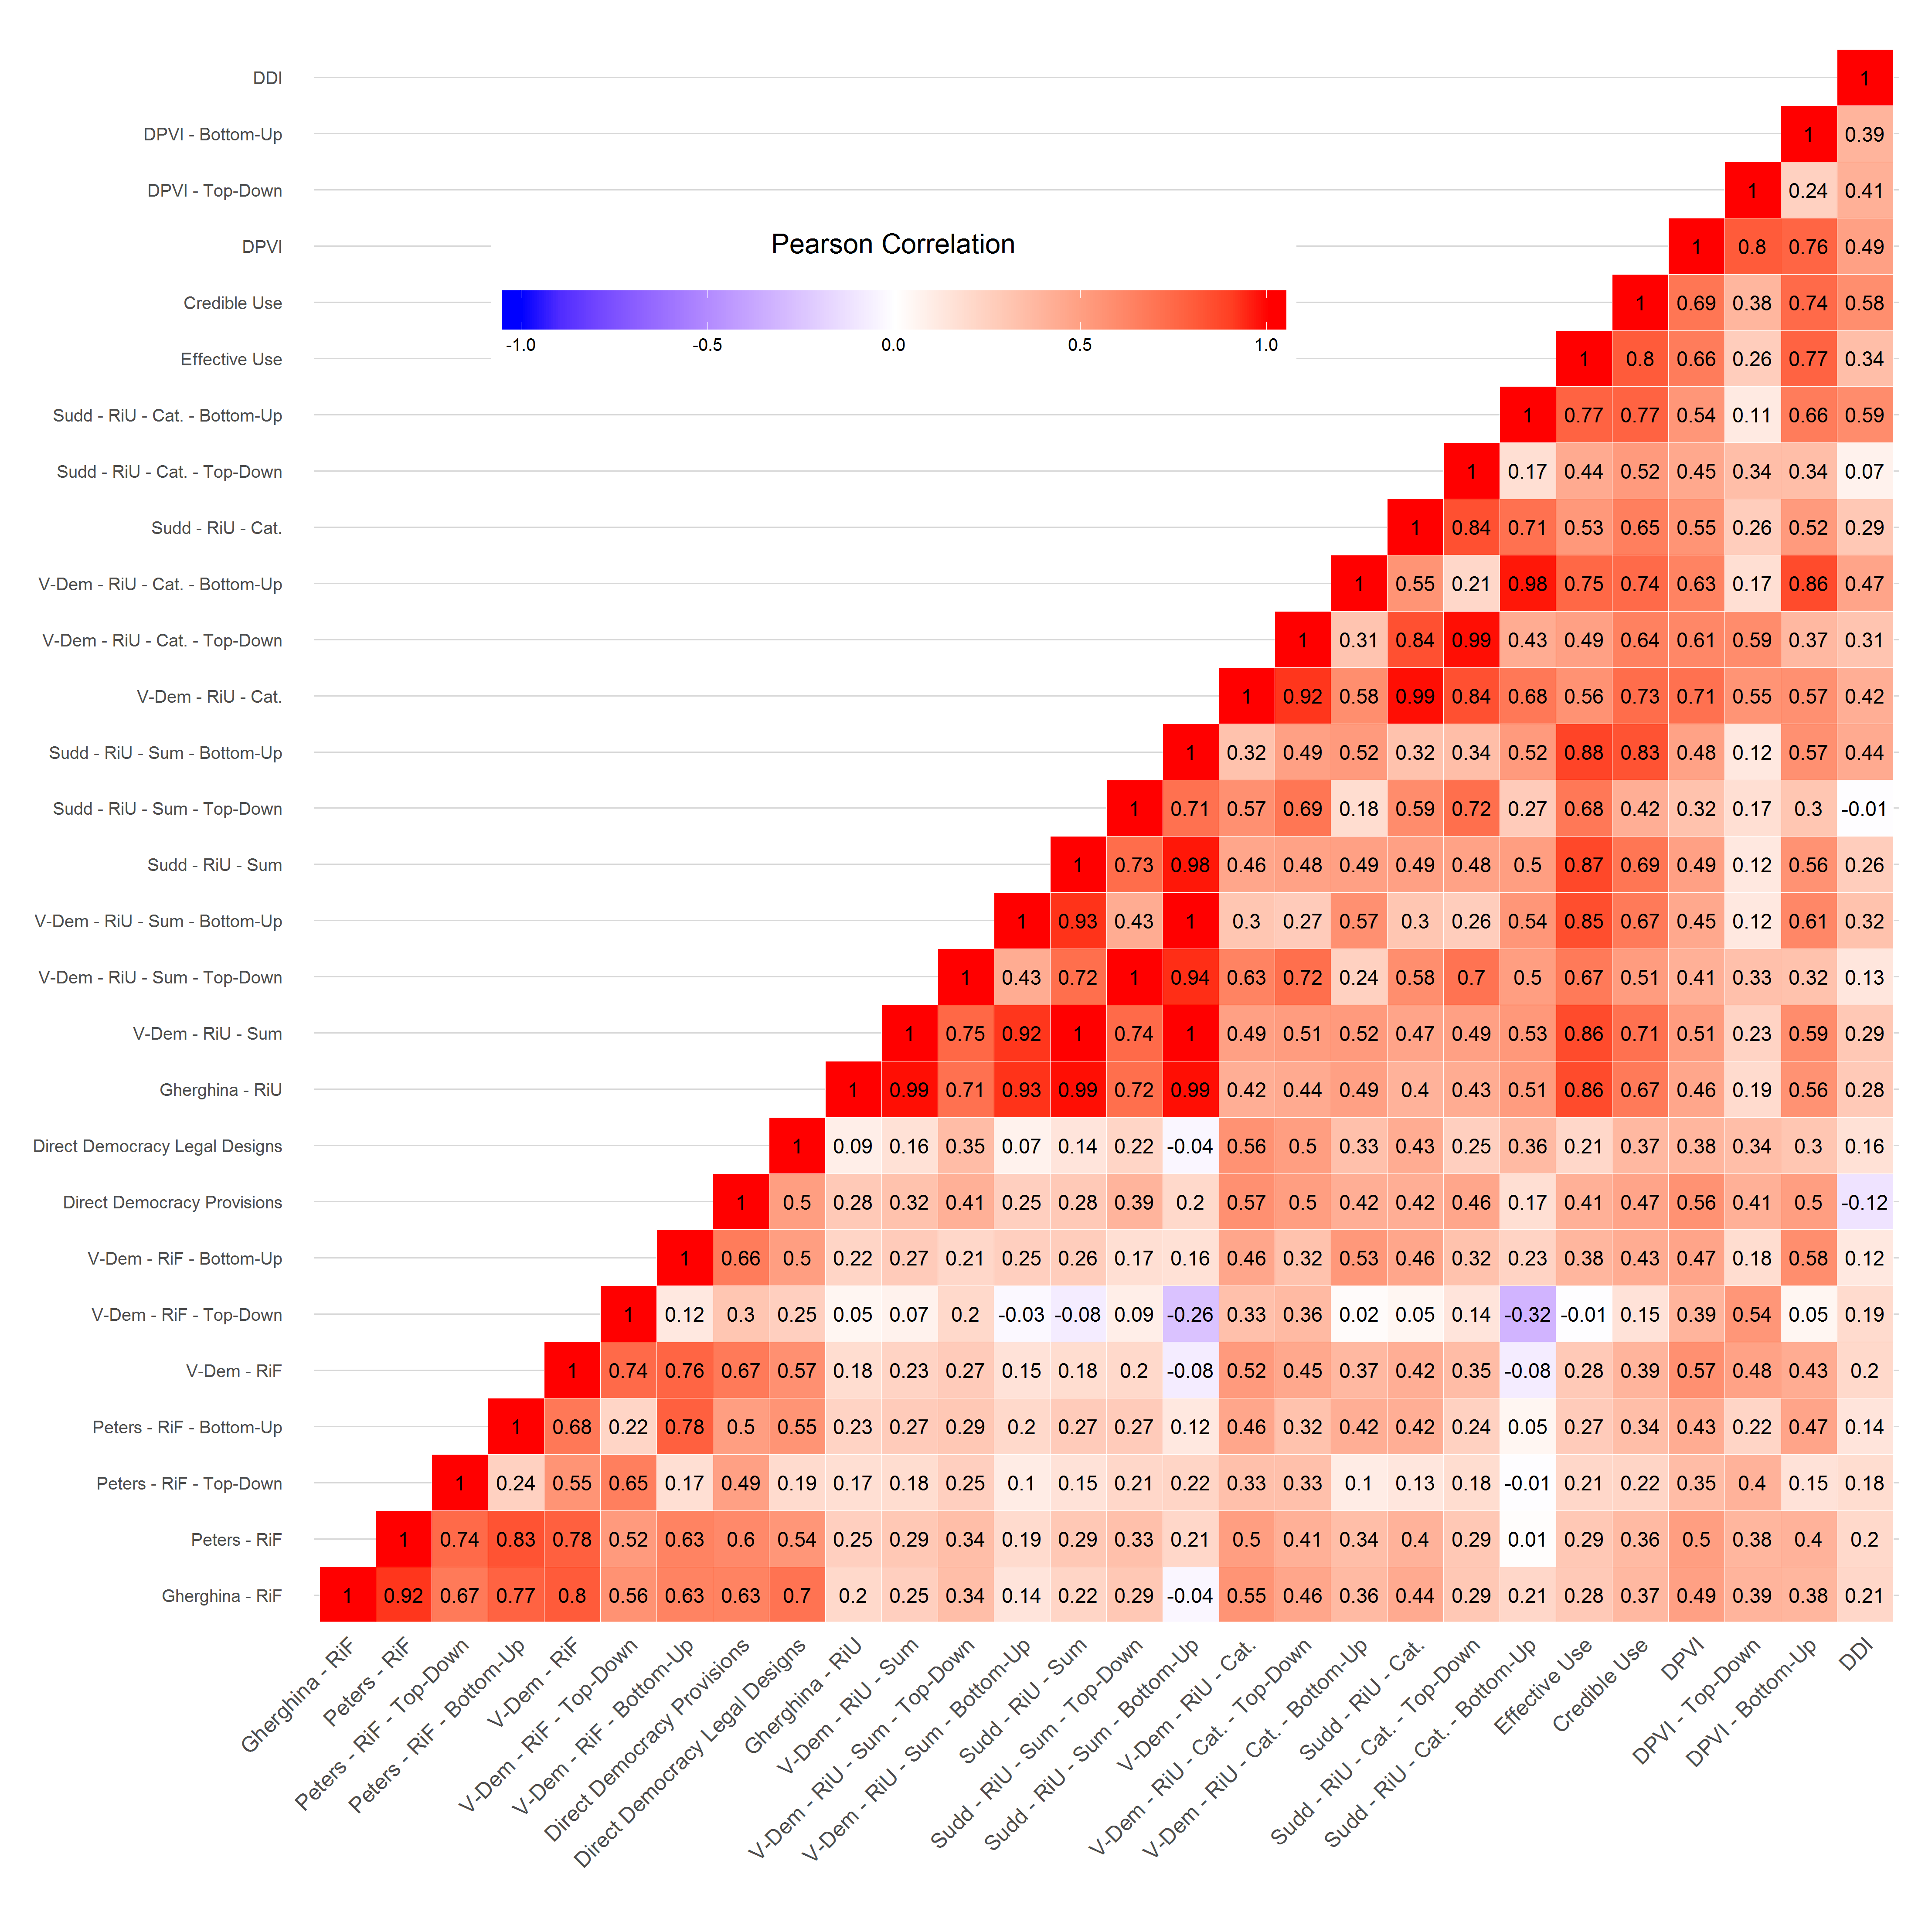
\includegraphics[width=\textwidth]{images/heatmap_fin.png}
	\flushright
	{\scriptsize Based on own calculations. Missing values excluded pairwise \par}
\end{figure}

\clearpage

\begin{table}[!ht]
	\centering
	\caption{Descritpion of Direct Democracy Index - Kaufmann}
	\label{kaufmann}
	\resizebox{\textwidth}{!}{%
		\begin{tabular}{@{}ll@{}}
			\toprule
			\multicolumn{1}{c}{\textbf{Score}} & \multicolumn{1}{c}{\textbf{Description}} \\ \midrule
			\textit{1.) The Radical Democrat} & \begin{tabular}[c]{@{}l@{}}Citizens have access to a broad spectrum of direct-democratic procedures. \\ As well as the binding popular initiative, these include the right of facultative referendum \\ and obligatory referendums for alterations to the Constitution and state treaties.\end{tabular} \\ \midrule
			\textit{2.) The Progressive} & \begin{tabular}[c]{@{}l@{}}Citizens have, at least in part, the possibility of initiating national referendums \\ without the express permission of the organs of the state (parliament, government, president). \\ There are also procedures for obligatory referendums.\end{tabular} \\ \midrule
			\textit{3.) The Cautious} & \begin{tabular}[c]{@{}l@{}}The electorate does have practical experience of popular initiatives and /or national referendums. \\ But these procedures are essentially plebiscitary in nature, i.e. they are not protected or controlled \\ by the citizens themselves or by the law, but are controlled “from above” by parliament (political parties) \\ or by the executive.\end{tabular} \\ \midrule
			\textit{4.) The Hesitant} & \begin{tabular}[c]{@{}l@{}}The political elites in the countries of this category appear to be afraid of popular participation in \\ political decision-making, whether out of fear of having to share power or because of concrete\\  historical experiences. Even here, however, there are still some traces of statutory I\&R procedures,\\ which may form the basis for future improvement .\end{tabular} \\ \midrule
			\textit{5.) The Fearful} & \begin{tabular}[c]{@{}l@{}}Almost entirely lacking institutional procedures and practical experience, \\ the countries in this category make it very hard for themselves to complement indirect democracy. \\ In addition, the political and cultural circumstances scarcely provide a stimulus for \\ the introduction or the strengthening of elements of popular decision-making. \\ Nonetheless, the issue is occasionally debated.\end{tabular} \\ \midrule
			\textit{6.) The Beginners} & \begin{tabular}[c]{@{}l@{}}These countries have only recently started their democratization process, \\ including a respect for basic freedoms and human rights. \\ Parliaments have been elected by the people, but there is still a great deal of mistrust \\ between governments and governed, making the introduction of additional instruments \\ like direct democracy extremely difficult. The Authoritarians: In the countries belonging \\ to this category, there is at present no basis at all for the development of direct democracy.\end{tabular} \\ \midrule
			\textit{7. The Authoritarians} & \begin{tabular}[c]{@{}l@{}}In the countries belonging to this category, \\ there is at present no basis at all for the development of direct democracy.\end{tabular} \\ \bottomrule
			\\[-1em]
\multicolumn{2}{r}{%
	\begin{minipage}{15cm}%
		\flushright
		\scriptsize Source: Kaufmann (2004)
	\end{minipage}%
}
		\end{tabular}%
	}
\end{table}



% \setcounter{table}{1}
% \renewcommand{\thetable}{B\arabic{table}}
% \setcounter{figure}{1}
% \renewcommand{\thefigure}{B\arabic{figure}}


%---------------------------------------------------------------------------%
% Eigenständigkeiterklärung
%---------------------------------------------------------------------------%
\clearpage
\section*{Eigenständigkeitserklärung}
\vspace*{2cm}
\begin{center}
	\begin{minipage}[t]{0.8\textwidth}
		Hiermit versichern wir, dass wir die vorliegende Hausarbeit selbständig und nur mit den angegebenen Hilfsmitteln verfasst haben. Alle Passagen, die wir wörtlich als auch sinngemäß aus der Literatur oder aus anderen Quellen wie z. B. Internetseiten entnommen haben, sind deutlich als Zitat mit Angabe der Quelle kenntlich gemacht.
		
		\vspace*{60mm}
		Stuttgart, 03.03.2018
	\end{minipage}
\end{center}


\end{document}

